% !TeX root = RJwrapper.tex
\title{Partitioned Local Depth (PaLD) Community Analyses in R}
\author{by Lucy D'Agostino McGowan, Katherine Moore, and Kenneth Berenhaut}

\maketitle

\abstract{%
Partitioned Local Depth (PaLD) is a framework for a holistic
consideration of the community structure of distance-based data. This
paper describes an R package, \CRANpkg{pald}, for calculating
Partitioned Local Depth (PaLD) probabilities, implementing community
analyses, and creating data visualizations to display community
structure. We describe how to use the package as well as walk through
several examples.
}

\hypertarget{introduction}{%
\subsection{Introduction}\label{introduction}}

Partitioned Local Depth (PaLD) is a framework for a holistic
consideration of community structure for distance-based data. Leveraging
a socially inspired perspective, the method provides network-based
community information which is founded on a new measure of local depth
and pairwise cohesion (partitioned local depth). The method does not
require distributional assumptions, optimization criteria, nor
extraneous inputs. A complete description of the perspective, together
with a discussion of the underlying social motivation, theoretical
results, and applications to additional data sets is provided in
\citet{berenhaut2022social}.

Building on existing approaches to (global) depth, local depth expresses
features of centrality via an interpretable probability which is free of
parameters and robust to outliers. Then, partitioning the probability
which defines local depth, we obtain a measure of cohesion between pairs
of points. Both local depth and cohesion reflect aspects of relative
position (rather than absolute distance) and provide a straightforward
way to account for varying density across the space. Specifically, as
shown in \citet{berenhaut2022social}, provided that two sets are
separated (in the sense that the minimum between-set distance is greater
than the maximum within-set distance), cohesion is invariant under the
contraction and dilation of the distances within each set. This property
may be particularly valuable when one has reason to believe that there
is heterogeneity in density across the space.

As cohesion captures a sense of the relationship strength between
points, we can then visualize the resulting community structure with a
network whose edges are weighted by (mutual) cohesion. The underlying
social framework motivates a straightforward yet elegant threshold for
distinguishing between strongly and weakly cohesive pairs.

Throughout this paper, we will display the network obtained from
cohesion using a force-directed graph drawing algorithm and emphasize
the strong ties (colored by connected component). We refer to the
connected components of the network of strong ties as community
``clusters.'' Note that to qualify as a cluster in this definition, one
may not have any strong ties with those outside the cluster, and thus
the existence of disjoint groups is a strong signal for separation.
Here, clusters are identified without additional user inputs nor
optimization criteria. If one wishes to further break the community
graph into groups, one may consider using community detection methods
(such as spectral clustering or the Louvain algorithm), as available,
say, in the \CRANpkg{igraph} package. Though only briefly considered
here, one may also use the collection of strong ties in place of
(weighted) k-nearest neighbors in settings such as classification and
smoothing. Overall, the structural information obtained from local
depth, cohesion and community graphs can provide a holistic perspective
on the data which does not require the use of distributional
assumptions, optimization criteria nor additional user inputs.

We present a new package, \CRANpkg{pald}, for calculating Partitioned
Local Depth (PaLD) probabilities, implementing community analyses, and
creating data visualizations to display community structure. This paper
will describe how to use the package, walk through several examples, and
compare the method to commonly used techniques in R. Together, these
demonstrate both the novelty of the method and utility of the
implementation in package described.

\hypertarget{pald}{%
\subsection{pald}\label{pald}}

The main functions in the \CRANpkg{pald} package can be split into 3
categories:

\begin{enumerate}
\def\labelenumi{\arabic{enumi}.}
\tightlist
\item
  A function for computing the cohesion matrix
\item
  Functions for extracting useful information from the cohesion matrix,
  such as local depths, neighbors, community clusters, and graph objects
\item
  Plotting functions for community graphs
\end{enumerate}

In addition, the package provides a number of pertinent example data
sets commonly used to demonstrate cluster algorithms, including a
synthetic data set of two-dimensional points created by
\citet{gionis1clustering} to demonstrate clustering aggregation,
clustering data generated from the scikit-learn Python package
\citep{pedregosa2011scikit}, data describing cognate relationships
between words across 87 Indo-European languages \citep{dyen92}, data
compiled by \cite{tissue} of tissue gene expressions, data from the
World Values Survey \citep{inglehart2014world} on cultural values
regarding family, religion, education, and institutions for several
regions \citep{muthukrishna2020beyond}, and three example data sets
generated for the \citet{berenhaut2022social} paper.

While it is not a necessity, the \CRANpkg{pald} package is designed to
function well with the pipe operator, \texttt{\textbar{}\textgreater{}}.
This functionality will be demonstrated below.

\hypertarget{creating-the-cohesion-matrix}{%
\subsubsection{Creating the cohesion
matrix}\label{creating-the-cohesion-matrix}}

The input for the Partitioned Local Depths (PaLD) computations is a
distance matrix or \texttt{dist} object. Note that the collection of
input distances (or dissimilarities) does not need to satisfy the
triangle inequality nor be symmetric.

For demonstration purposes, we will show how one can compute a distance
matrix from an input data frame with, say, two variables \texttt{x1} and
\texttt{x2}. The input data may be of any dimension; in fact the PaLD
framework provides advantages when considering high-dimensional data
(see the \textbf{Examples} section as well as
\citet{berenhaut2022social}).

\begin{Schunk}
\begin{Sinput}
library(pald)
df <- data.frame(
  x1 = c(6, 8, 8, 16, 4, 14),
  x2 = c(5, 4, 10, 8, 4, 10)
)
rownames(df) <- c("A", "B", "C", "D", "E", "F")
\end{Sinput}
\end{Schunk}

The \texttt{dist()} function converts an input data frame into a
distance matrix, as demonstrated below. If the data are already provided
as a distance matrix (or \texttt{dist} object), the user can skip to the
next step. Note that the distance matrix needed for the subsequent
functions doesn't need to be a \texttt{dist} object and \emph{need not}
be symmetric.

\begin{Schunk}
\begin{Sinput}
d <- dist(df)
\end{Sinput}
\end{Schunk}

The function above creates a \texttt{dist} object. If converted to a
matrix, this will be an \(n\times n\) distance matrix, where \(n\)
corresponds to the number of observations in the original data frame, in
this example \(n = 6\).

This \texttt{dist} object, or a distance matrix, can then be passed to
the \texttt{cohesion\_matrix()} function in order to calculate the
pairwise cohesion values.

Cohesion is an interpretable probability that reflects the strength of
alignment of two points within local regions. It captures aspects of the
relative positioning of points and accounts for varying density across
the space.

\begin{Schunk}
\begin{Sinput}
d <- dist(df)
cohesion_matrix(d)
\end{Sinput}
\begin{Soutput}
#>            A          B          C         D          E         F
#> A 0.25000000 0.18333333 0.06666667 0.0000000 0.18333333 0.0000000
#> B 0.14000000 0.24000000 0.05000000 0.0000000 0.10666667 0.0000000
#> C 0.07333333 0.07333333 0.20333333 0.0000000 0.03333333 0.0800000
#> D 0.00000000 0.00000000 0.00000000 0.2333333 0.00000000 0.1333333
#> E 0.14000000 0.10666667 0.03333333 0.0000000 0.24000000 0.0000000
#> F 0.00000000 0.00000000 0.05000000 0.1400000 0.00000000 0.2400000
#> attr(,"class")
#> [1] "cohesion_matrix" "matrix"          "array"
\end{Soutput}
\end{Schunk}

Equivalently, the user can use the native pipe
\texttt{\textbar{}\textgreater{}} as follows.

\begin{Schunk}
\begin{Sinput}
df |>
  dist() |>
  cohesion_matrix()
\end{Sinput}
\begin{Soutput}
#>            A          B          C         D          E         F
#> A 0.25000000 0.18333333 0.06666667 0.0000000 0.18333333 0.0000000
#> B 0.14000000 0.24000000 0.05000000 0.0000000 0.10666667 0.0000000
#> C 0.07333333 0.07333333 0.20333333 0.0000000 0.03333333 0.0800000
#> D 0.00000000 0.00000000 0.00000000 0.2333333 0.00000000 0.1333333
#> E 0.14000000 0.10666667 0.03333333 0.0000000 0.24000000 0.0000000
#> F 0.00000000 0.00000000 0.05000000 0.1400000 0.00000000 0.2400000
#> attr(,"class")
#> [1] "cohesion_matrix" "matrix"          "array"
\end{Soutput}
\end{Schunk}

The \emph{cohesion matrix} output by the \texttt{cohesion\_matrix()}
function is the main input for the majority of the remaining functions.

\hypertarget{functions-for-extracting-information-from-the-cohesion-matrix}{%
\subsubsection{Functions for extracting information from the cohesion
matrix}\label{functions-for-extracting-information-from-the-cohesion-matrix}}

From the \emph{cohesion matrix}, a variety of useful quantities can be
computed. Below, we create a cohesion matrix using the functions
described in the previous section.

\begin{Schunk}
\begin{Sinput}
df |>
  dist() |>
  cohesion_matrix() -> cohesion
\end{Sinput}
\end{Schunk}

The \texttt{local\_depths()} function calculates the \emph{depth} of
each point, outputting a vector of local depths. Local depth is an
interpretable probability which reflects aspects of relative position
and centrality via distance comparisons (i.e., \(d(z, x) < d(z, y)\),
see \citet{berenhaut2022social}).

\begin{Schunk}
\begin{Sinput}
local_depths(cohesion)
\end{Sinput}
\begin{Soutput}
#>         A         B         C         D         E         F 
#> 0.6833333 0.5366667 0.4633333 0.3666667 0.5200000 0.4300000
\end{Soutput}
\end{Schunk}

In this case, the deepest point is \texttt{A}.

The \texttt{strong\_threshold()} function will calculate the cohesion
threshold for strong ties. This is equal to half the average of the
diagonal of the cohesion matrix \citep{berenhaut2022social}, and is a
threshold that may be used to distinguish between strong and weak ties.

\begin{Schunk}
\begin{Sinput}
strong_threshold(cohesion)
\end{Sinput}
\begin{Soutput}
#> [1] 0.1172222
\end{Soutput}
\end{Schunk}

In this case, the threshold is a little above \texttt{0.117}.

The function \texttt{cohesion\_strong()} will update the cohesion matrix
to set all weak ties to zero (via the \texttt{strong\_threshold()}
function). Optionally, the matrix will also be symmetrized, using the
entry-wise (parallel) minimum of the cohesion matrix and its transpose,
with the default parameter \texttt{symmetric\ =\ TRUE}.

\begin{Schunk}
\begin{Sinput}
cohesion_strong(cohesion)
\end{Sinput}
\begin{Soutput}
#>      A    B         C         D    E         F
#> A 0.25 0.14 0.0000000 0.0000000 0.14 0.0000000
#> B 0.14 0.24 0.0000000 0.0000000 0.00 0.0000000
#> C 0.00 0.00 0.2033333 0.0000000 0.00 0.0000000
#> D 0.00 0.00 0.0000000 0.2333333 0.00 0.1333333
#> E 0.14 0.00 0.0000000 0.0000000 0.24 0.0000000
#> F 0.00 0.00 0.0000000 0.1333333 0.00 0.2400000
#> attr(,"class")
#> [1] "cohesion_matrix" "matrix"          "array"
\end{Soutput}
\end{Schunk}

The \texttt{community\_graphs()} function takes the cohesion matrix and
creates \CRANpkg{igraph} objects, graphs that describe the relationship
between the points. This function will output a list of three objects:

\begin{itemize}
\tightlist
\item
  \texttt{G}: the weighted (community) graph whose edge weights are
  mutual cohesion
\item
  \texttt{G\_strong}: the weighted (community) graph consisting of edges
  for which mutual (symmetrized) cohesion (i.e.~the minimum of the two
  directed cohesion values for any given pair) is greater than the
  threshold for strong ties
\item
  \texttt{layout}: the graph layout, using the Fruchterman Reingold (FR)
  force-directed graph drawing for the graph \texttt{G}
\end{itemize}

\begin{Schunk}
\begin{Sinput}
graphs <- community_graphs(cohesion)
graphs[["G_strong"]]
\end{Sinput}
\begin{Soutput}
#> IGRAPH f9306e2 UNW- 6 3 -- 
#> + attr: name (v/c), weight (e/n)
#> + edges from f9306e2 (vertex names):
#> [1] A--B A--E D--F
\end{Soutput}
\end{Schunk}

Here we see that there are three connected components, ties \texttt{A-B}
and \texttt{A-E} which form the first cluster, and the tie \texttt{D-F}
which forms another.

The \texttt{any\_isolated()} function will check whether there are any
isolated points.

\begin{Schunk}
\begin{Sinput}
any_isolated(cohesion)
\end{Sinput}
\end{Schunk}

\noindent Here, there are no isolated points, i.e.~points having zero
cohesion with all other points in the data (an extreme form of outlier).

The ``community clusters'' identified by PaLD are the connected
components of the graph of strong ties, \texttt{G\_strong}. To directly
calculate them, we can use the \texttt{community\_clusters()} function.
This will output a data frame with two columns, the first will
correspond to the \texttt{point}, as identified by the row name of the
original input data frame, \texttt{df}, the second will identify the
\texttt{cluster} that each point belongs to.

\begin{Schunk}
\begin{Sinput}
community_clusters(cohesion)
\end{Sinput}
\begin{Soutput}
#>   point cluster
#> A     A       1
#> B     B       1
#> C     C       2
#> D     D       3
#> E     E       1
#> F     F       3
\end{Soutput}
\end{Schunk}

In this example, three clusters are identified with these six points.
Points \texttt{A}, \texttt{B}, and \texttt{E} fall into cluster 1. Point
\texttt{C} is in cluster 2 (a cluster of size 1) and points \texttt{D}
and \texttt{F} fall into cluster 3.

\hypertarget{plotting-functions}{%
\subsection{Plotting functions}\label{plotting-functions}}

The final category of function is that for data visualization. We can
begin by visualizing the points in the data frame \texttt{df} (Figure
\ref{fig:fig1}). When visualizing these points, it is important to have
the aspect ratio of the x and y axes equal to 1 so as to not distort
distances. When using the \CRANpkg{ggplot2} package for this
visualization, one can use the \texttt{coord\_fixed(ratio\ =\ 1)}
function. If using the \texttt{plot()} function included in the base
library, one can use the \texttt{asp\ =\ 1} argument.

\begin{Schunk}
\begin{Sinput}
library(ggplot2)
ggplot(df, aes(x1, x2)) +
  geom_text(label = rownames(df)) + 
  coord_fixed(ratio = 1) + 
  xlim(c(4, 16)) + 
  ylim(c(4, 16))
\end{Sinput}
\begin{figure}
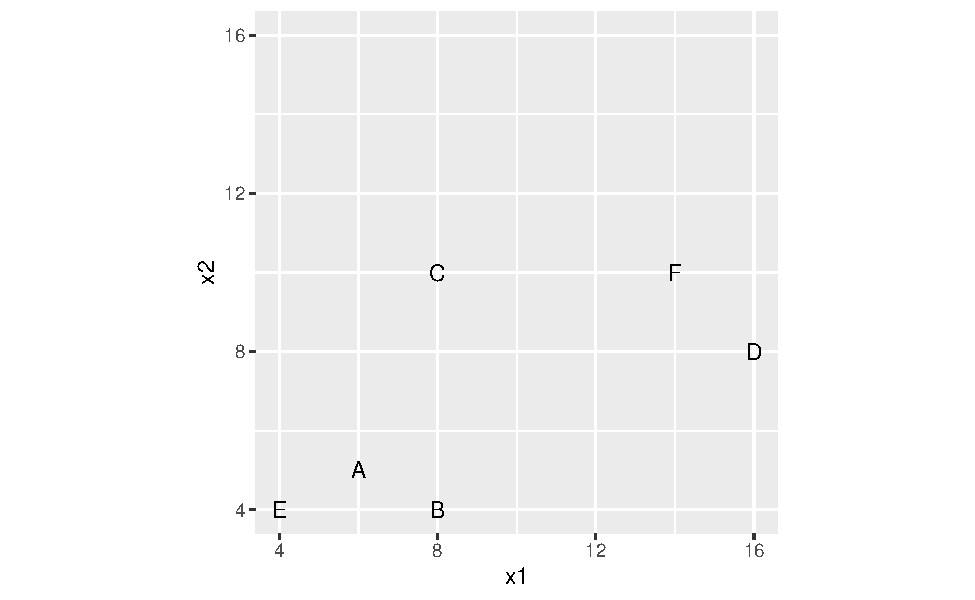
\includegraphics{dagostino-mcgowan_files/figure-latex/fig1-1} \caption[Visualization of the points from the data frame `df`]{Visualization of the points from the data frame `df`}\label{fig:fig1}
\end{figure}
\end{Schunk}

We can pass the cohesion matrix to the
\texttt{plot\_community\_graphs()} function to view the relationship
between points (Figure \ref{fig:fig2}). Notice in this plot the layout
does not match that of the original data frame as seen in Figure
\ref{fig:fig1}. Since our original data is two dimensional, it may be
reasonable to use this as the layout. Figure \ref{fig:fig3} will make
this update as well as update some of the aesthetics, such as employing
more readable labels.

\begin{Schunk}
\begin{Sinput}
plot_community_graphs(cohesion)
\end{Sinput}
\begin{figure}
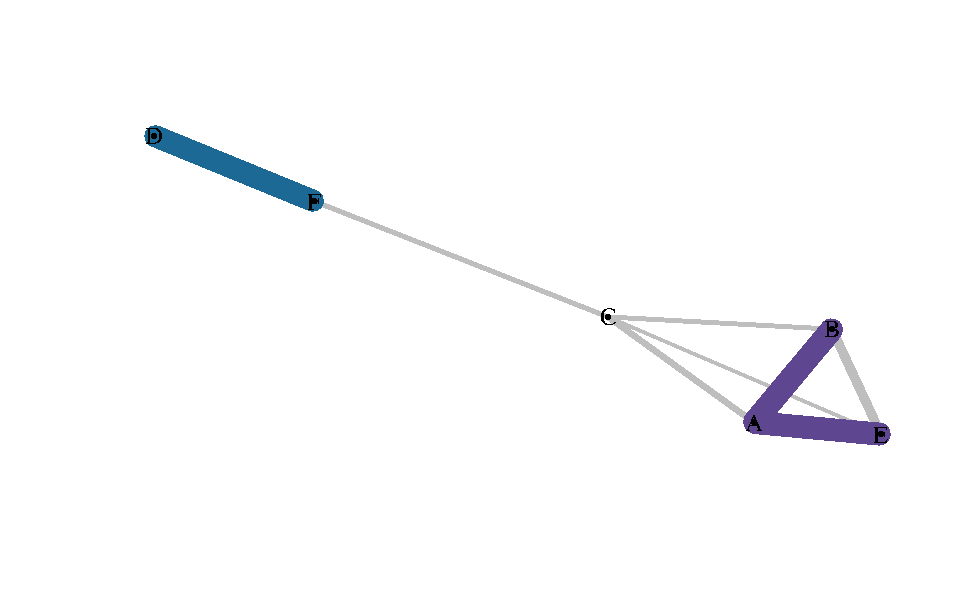
\includegraphics{dagostino-mcgowan_files/figure-latex/fig2-1} \caption[PaLD graph displaying the relationship between the points in data frame `df`]{PaLD graph displaying the relationship between the points in data frame `df`}\label{fig:fig2}
\end{figure}
\end{Schunk}

The \texttt{layout} argument allows the user to pass a matrix to dictate
the 2-dimensional layout of the graph. For example, if we wanted the
graph to match the visualization displayed in Figure \ref{fig:fig1}, we
could pass \texttt{as.matrix(df)}, or a matrix of the data frame
\texttt{df} to the \texttt{layout} argument (Figure \ref{fig:fig3}).
Additionally, the \texttt{plot\_community\_graphs()} function will also
permit parameters that can be passed to the \texttt{plot.igraph()}
function. We can pass arguments to the \texttt{plot.igraph} function via
the \texttt{...} argument; for example to increase the vertex size and
change the vertex label color, we can specify
\texttt{vertex.size\ =\ 100} and
\texttt{vertex.label.color\ =\ "white"}. Additionally, to allow axes, we
use \texttt{axes\ =\ TRUE}, and to put them back on the original scale
we set \texttt{rescale\ =\ FALSE}, resetting the axis limits using
\texttt{xlim} and \texttt{ylim}. The \texttt{par(pty\ =\ "s")} function
forces the subsequent plot to be square.

\begin{Schunk}
\begin{Sinput}
par(pty = "s")

plot_community_graphs(cohesion, 
                      layout = as.matrix(df),
                      vertex.size = 100,
                      vertex.label.color = "white",
                      axes = TRUE,
                      rescale = FALSE,
                      asp = 1,
                      xlim = c(4, 16),
                      ylim = c(4, 16))
\end{Sinput}
\begin{figure}
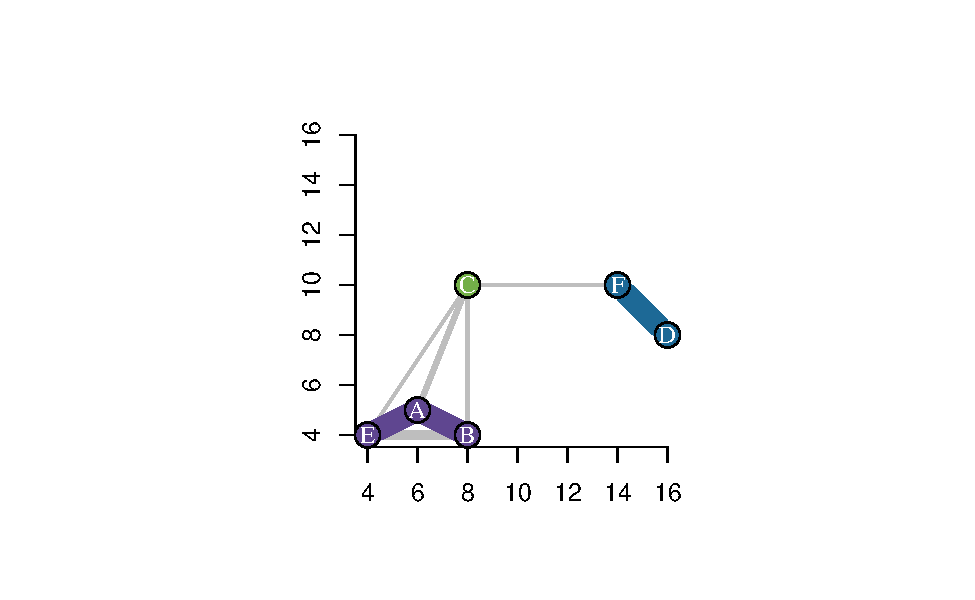
\includegraphics{dagostino-mcgowan_files/figure-latex/fig3-1} \caption[PaLD graph displaying the relationship between the points in data frame `df`, matching the original layout in Figure 1]{PaLD graph displaying the relationship between the points in data frame `df`, matching the original layout in Figure 1}\label{fig:fig3}
\end{figure}
\end{Schunk}

\hypertarget{examples}{%
\subsection{Examples}\label{examples}}

We will demonstrate the utility of the \CRANpkg{pald} package in three
illustrative examples.

\hypertarget{clustering-tissue-gene-expression-data}{%
\subsubsection{Clustering tissue gene expression
data}\label{clustering-tissue-gene-expression-data}}

The first example is from a subset of data from \citet{zilliox2007gene},
\citet{mccall2011gene}, and \citet{mccall2014gene}, obtained from the
\textbf{tissuesGeneExpression} bioconductor package \citep{tissue}
consisting of 22,215-dimensional gene expression data from 189 tissue
samples. A \texttt{dist} object was created using this data set and is
included in the \CRANpkg{pald} package in an object called
\texttt{tissue\_dist}.

The \texttt{tissue\_dist} object is a \texttt{dist} object resulting in
a distance matrix with 189 rows and 189 columns.

We can create the cohesion matrix using the \texttt{cohesion\_matrix}
function.

\begin{Schunk}
\begin{Sinput}
tissue_cohesion <- cohesion_matrix(tissue_dist)
\end{Sinput}
\end{Schunk}

The \texttt{community\_clusters()} function can be used to identify the
community cluster corresponding to each tissue sample. Since the output
is a data frame, we can summarize the result using commonly employed
data analysis techniques. For demonstration purposes, we will use the
\CRANpkg{dplyr} package to summarize the contribution of clusters.

\begin{Schunk}
\begin{Sinput}
community_clusters(tissue_cohesion) |>
  dplyr::count(cluster, point)
\end{Sinput}
\begin{Soutput}
#>    cluster       point  n
#> 1        1 endometrium 15
#> 2        1      kidney 39
#> 3        2 hippocampus 31
#> 4        3  cerebellum 26
#> 5        4  cerebellum  1
#> 6        5       colon 33
#> 7        6       colon  1
#> 8        7       liver  7
#> 9        8  cerebellum  1
#> 10       9       liver 17
#> 11      10  cerebellum  2
#> 12      11       liver  2
#> 13      12  cerebellum  1
#> 14      13  cerebellum  4
#> 15      14  cerebellum  2
#> 16      15  cerebellum  1
#> 17      16    placenta  2
#> 18      17    placenta  1
#> 19      18    placenta  3
\end{Soutput}
\end{Schunk}

From this, we can glean that cluster 1 consists of two types of tissue,
the kidney and endometrium. Cluster 2 is comprised of only the
hippocampus.

We can also display the relationships between tissue samples using the
\texttt{plot\_community\_graphs()} function (Figure \ref{fig:fig4}). For
clarity of the display, we show how to remove the labels using
\texttt{show\_labels\ =\ FALSE}. We will instead color by the labels by
passing these to the \texttt{vertex.color} parameter to the
\texttt{plot.igraph} function (via the \texttt{...} argument).
Similarly, we can add a legend using the \texttt{legend()} function, as
you would for an \CRANpkg{igraph} visualization. Additionally, we use
the \texttt{edge\_width\_factor} and \texttt{emph\_strong} arguments to
adjust the width of the lines between and within PaLD clusters.

\begin{Schunk}
\begin{Sinput}
labels <- rownames(tissue_cohesion)
plot_community_graphs(tissue_cohesion,
                      show_labels = FALSE,
                      vertex.size = 4,
                      vertex.color = as.factor(labels),
                      edge_width_factor = 35,
                      emph_strong = 5) 
legend("topleft", 
       legend = unique(as.factor(labels)), 
       pt.bg = unique(as.factor(labels)),
       col = "black",
       pch = 21)
\end{Sinput}
\end{Schunk}

\begin{Schunk}
\begin{figure}
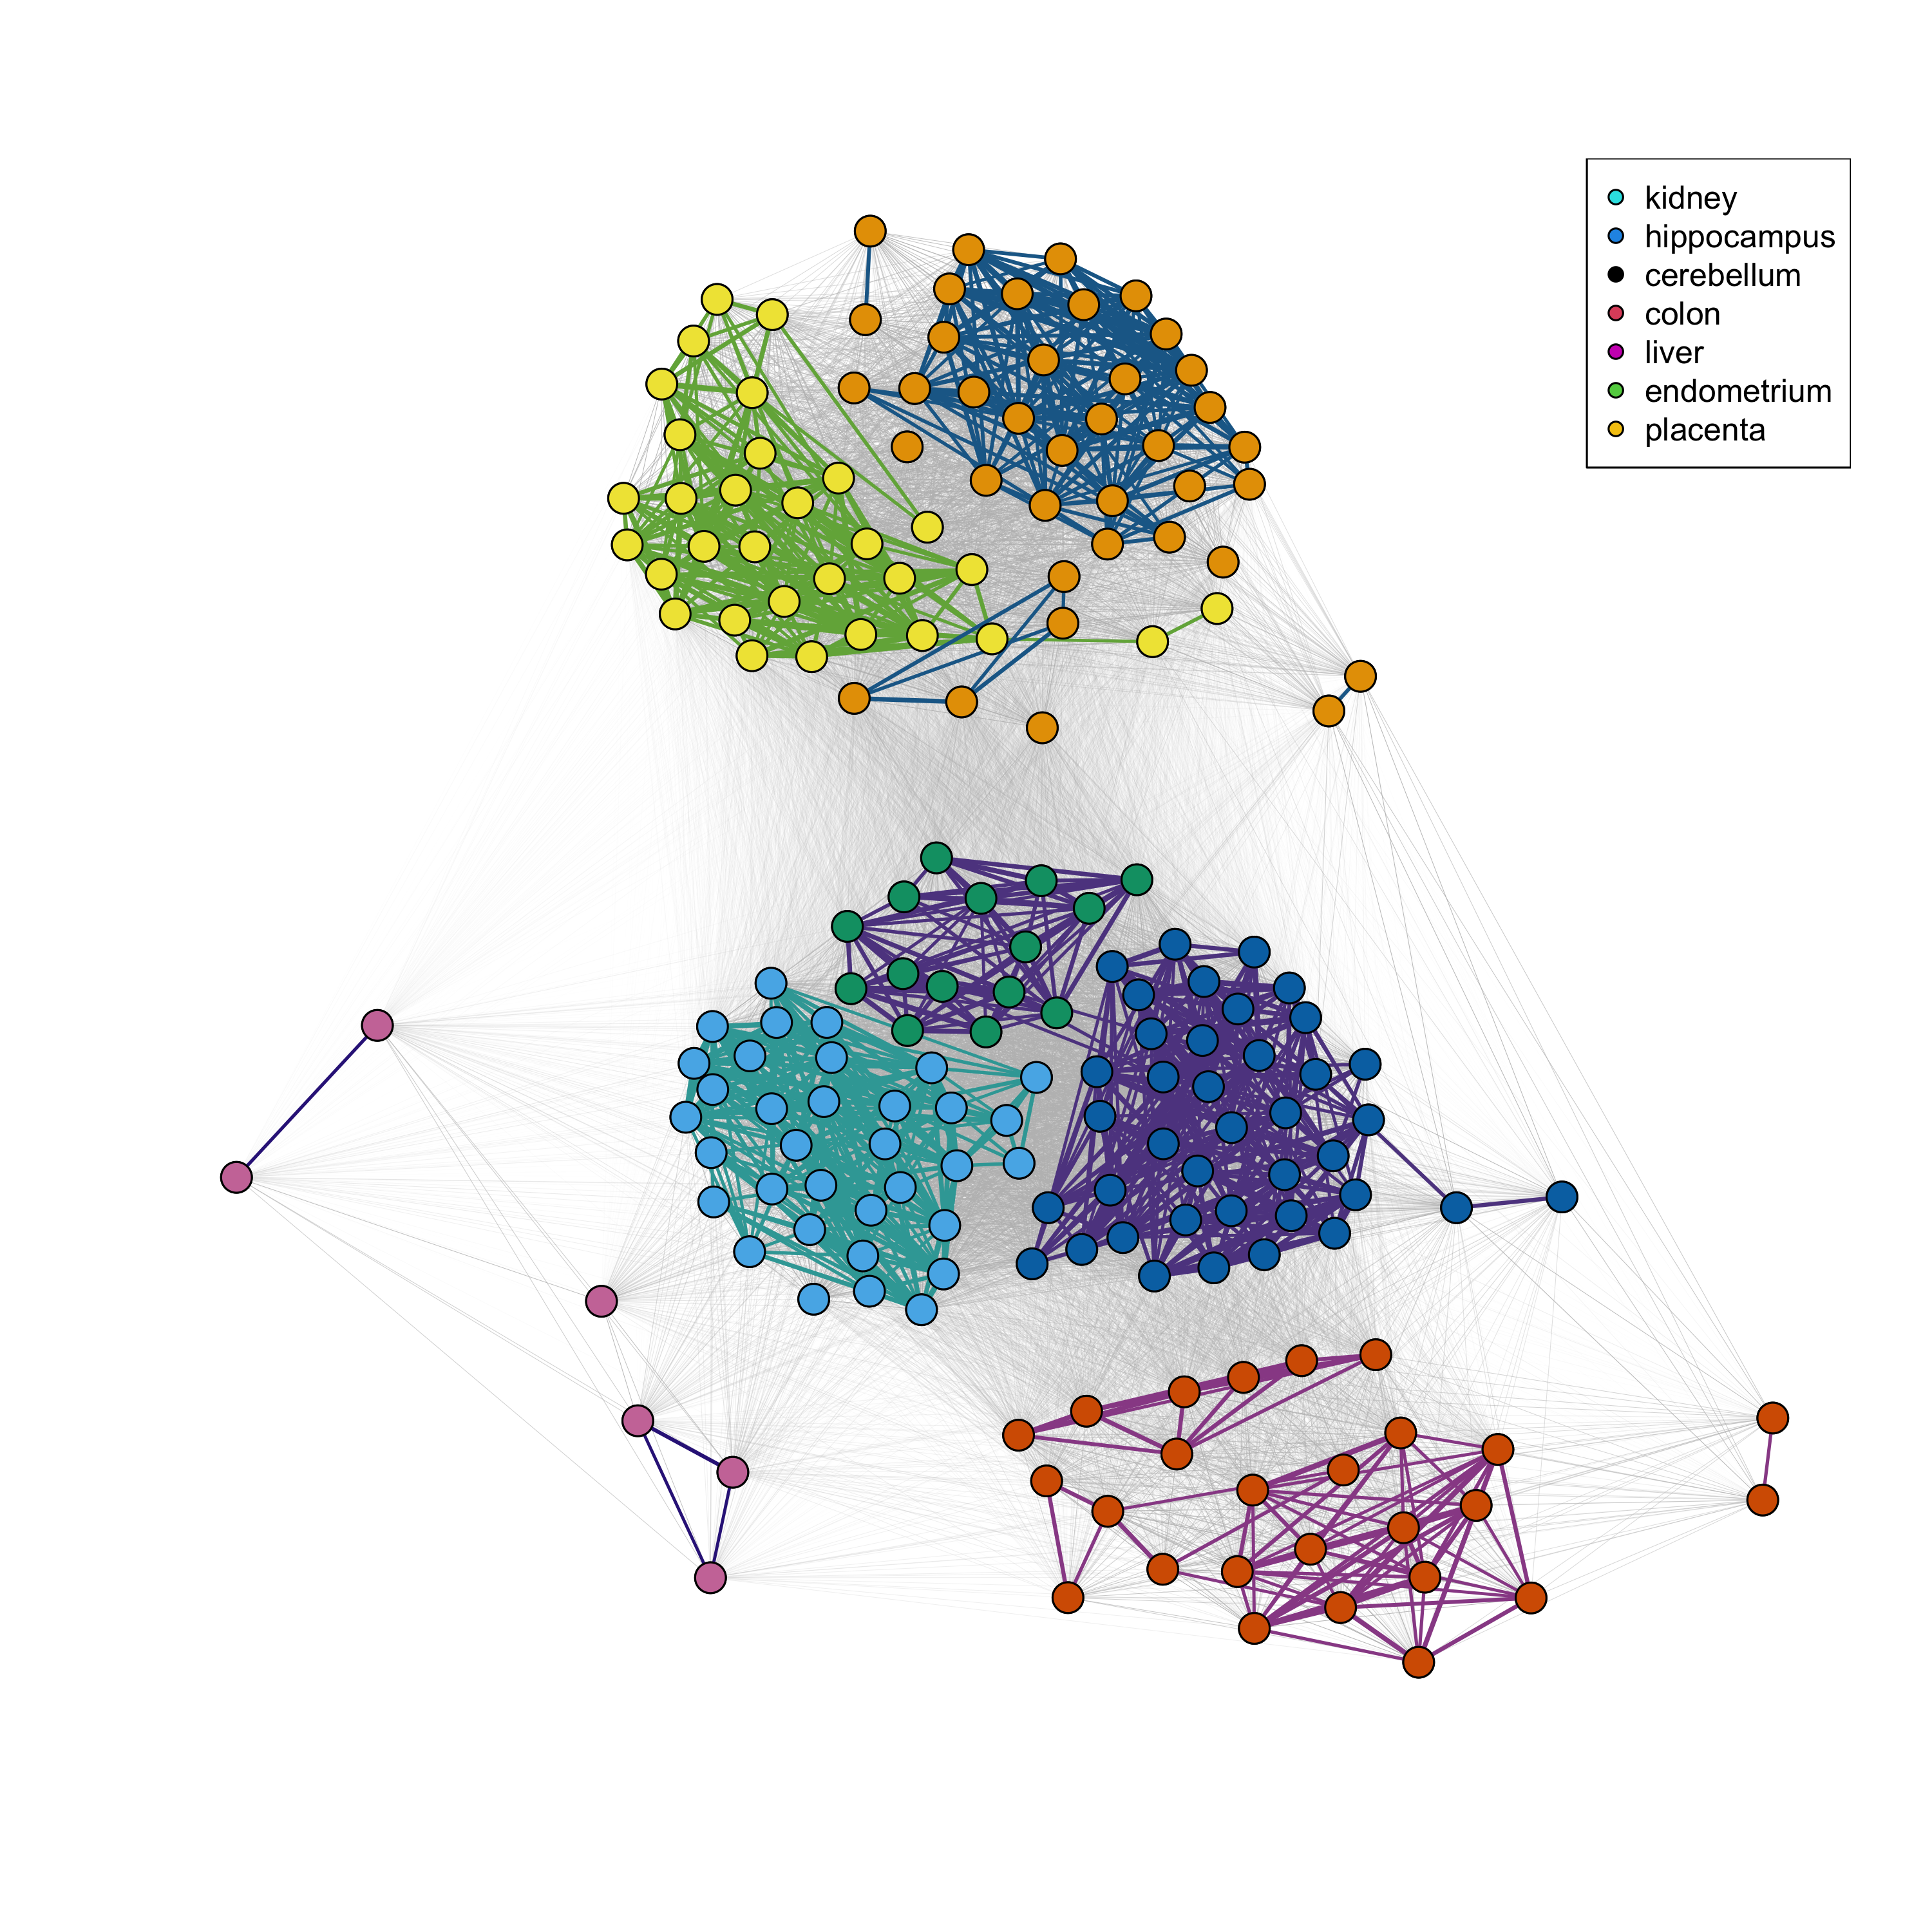
\includegraphics[width=1\linewidth]{fig5} \caption[Community cluster network for the tissue data]{Community cluster network for the tissue data. The line colors indicate the PaLD clusters, the point colors indicate the tissue classification.}\label{fig:fig4}
\end{figure}
\end{Schunk}

\hypertarget{cognate-based-language-families}{%
\subsection{Cognate-based Language
Families}\label{cognate-based-language-families}}

This example performs a PaLD analysis on a data set from \citet{dyen92}
that examines the relationship between 87 Indo-European languages from
the perspective of cognates, coded using 2,655-dimensional binary
vectors. A \texttt{dist} object was created from this data set and is
included in the \CRANpkg{pald} package in an object called
\texttt{cognate\_dist}.

This example will demonstrate how you can apply functions in the
\CRANpkg{igraph} package to objects output from the \CRANpkg{pald}
package. We can first use the \texttt{cohesion\_matrix()} function to
calculate the cohesion matrix and the \texttt{community\_graphs()}
function to create a list with the weighted community graph, the
weighted community graph with only strong ties included, and the layout.
From this, we can extract the graph with only the strong ties, here
called \texttt{cognate\_graph\_strong}.

\begin{Schunk}
\begin{Sinput}
cognate_cohesion <- cohesion_matrix(cognate_dist)
cognate_graphs <- community_graphs(cognate_cohesion)

cognate_graph_strong <- cognate_graphs[["G_strong"]]
\end{Sinput}
\end{Schunk}

We can then use the \texttt{neighbors()} function from the
\CRANpkg{igraph} package to extract the strong neighbors in this graph.
For example, if we wanted to extract all neighbors for the language
``French'', we could run the following.

\begin{Schunk}
\begin{Sinput}
french_neighbors <- igraph::neighbors(cognate_graph_strong, "French")
french_neighbors
\end{Sinput}
\begin{Soutput}
#> + 8/87 vertices, named, from 2660ad9:
#> [1] Italian         Ladin           Provencal       Walloon        
#> [5] French_Creole_C French_Creole_D Spanish         Catalan
\end{Soutput}
\end{Schunk}

Similarly, we can print the associated neighborhood weights by
subsetting the cohesion matrix.

\begin{Schunk}
\begin{Sinput}
cognate_cohesion["French", french_neighbors]
\end{Sinput}
\begin{Soutput}
#>         Italian           Ladin       Provencal         Walloon French_Creole_C 
#>      0.01997696      0.02094596      0.02871174      0.03258771      0.02406057 
#> French_Creole_D         Spanish         Catalan 
#>      0.02406057      0.01679733      0.01859688
\end{Soutput}
\end{Schunk}

We can again use the \texttt{plot\_community\_graphs()} function to
visualize the community clusters (Figure \ref{fig:figlang}). One may
note the commonly identifiable language clusters and that, under a
slight rotation, some of the underlying geography is mirrored in the
plot.

\begin{Schunk}
\begin{Sinput}
plot_community_graphs(
  cognate_cohesion,
  edge_width_factor = 30,
  emph_strong = 3,
  vertex.size = 3,
  vertex.label.cex = 0.7,
  vertex.label.dist = 1
)
\end{Sinput}
\end{Schunk}

\begin{Schunk}
\begin{figure}
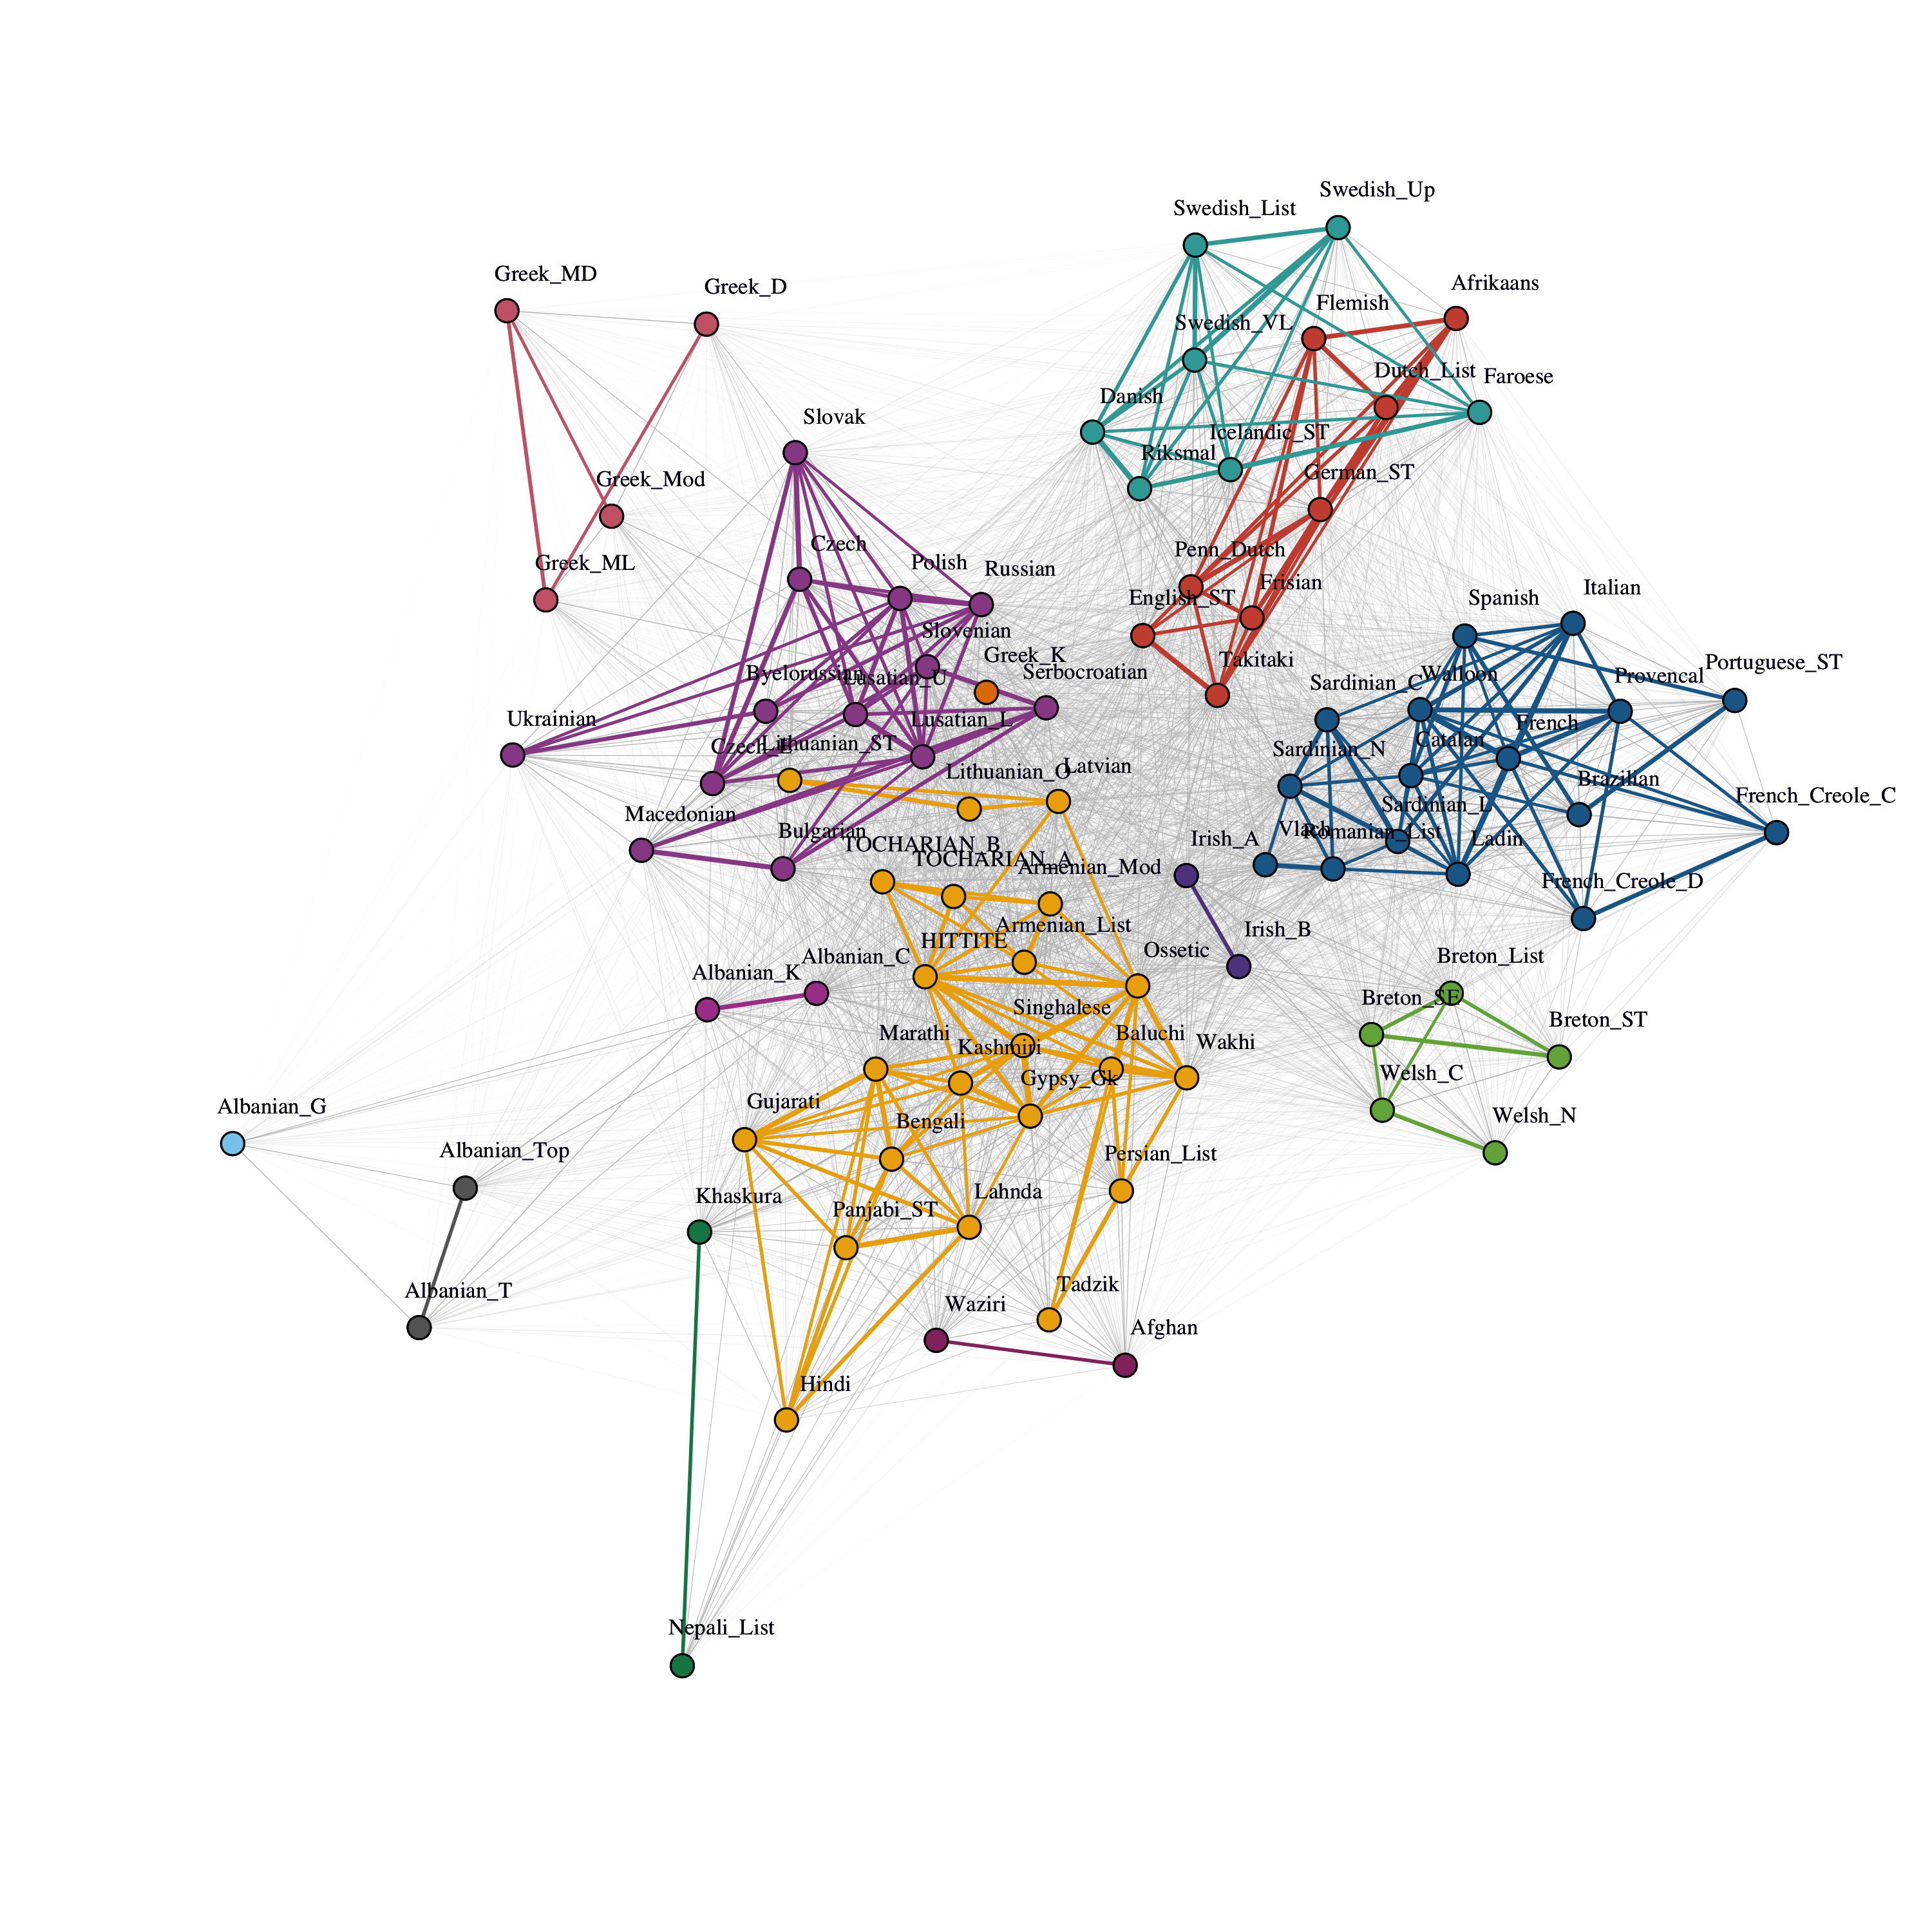
\includegraphics[width=1\linewidth]{fig6} \caption[Community structure for 87 Indo-European languages, which employs cognate information that was coded via 2,665-dimensional binary vectors]{Community structure for 87 Indo-European languages, which employs cognate information that was coded via 2,665-dimensional binary vectors. Commonly identifiable language clusters arise along with informative inter- and intra-cluster structure. Several ancient languages are centrally located.}\label{fig:figlang}
\end{figure}
\end{Schunk}

\hypertarget{community-analysis-for-generated-data}{%
\subsubsection{Community analysis for generated
data}\label{community-analysis-for-generated-data}}

The \CRANpkg{pald} package includes three randomly generated data frames
corresponding to plots from \citet{berenhaut2022social}:

\begin{itemize}
\tightlist
\item
  \texttt{exdata1} is a data set consisting of 8 points to recreate
  Figure 1 in \citet{berenhaut2022social}
\item
  \texttt{exdata2} is a data set consisting of 16 points to recreate
  Figure 2 in \citet{berenhaut2022social}
\item
  \texttt{exdata3} is a data set consisting of 240 points to recreate
  Figure 4D in \citet{berenhaut2022social}
\end{itemize}

Here, we will demonstrate how to use \texttt{exdata3}. These points were
generated from bivariate normal distributions with varying means and
variances. There are eight ``true'' communities.

We will demonstrate how we can compare PaLD to two clustering methods:
\emph{k}-means and hierarchical clustering. The code below calculates
the cohesion matrix (\texttt{exdata\_cohesion}) as well as the clusters
via PaLD (\texttt{exdata\_pald}), \emph{k}-means
(\texttt{exdata\_kmeans}) and hierarchical clustering using complete
linkage (\texttt{exdata\_hclust}).

\begin{Schunk}
\begin{Sinput}
exdata_cohesion <- exdata3 |>
  dist() |>
  cohesion_matrix()

exdata_pald <- community_clusters(exdata_cohesion)$cluster

exdata_kmeans <- kmeans(exdata3, 8)$cluster

exdata_hclust <- exdata3 |>
  dist() |>
  hclust() |>
  cutree(k = 8) 
\end{Sinput}
\end{Schunk}

We can compare this to the clustering generated by \emph{k}-means and
hierarchical clustering (Figure \ref{fig:fig5}).

\begin{Schunk}
\begin{Sinput}
par(mfrow = c(1, 3), pty = "s")
plot(
  exdata3,
  pch = 16,
  col = pald_colors[exdata_pald],
  xlab = "",
  ylab = "",
  main = "PaLD Clusters",
  asp = 1
)
plot(
  exdata3,
  pch = 16,
  col = pald_colors[exdata_kmeans],
  xlab = "",
  ylab = "",
  main = "K-Means Clusters (k = 8)",
  asp = 1
)
plot(
  exdata3,
  pch = 16,
  col = pald_colors[exdata_hclust],
  xlab = "",
  ylab = "",
  main = "Hiearchical Clusters (k = 8)",
  asp = 1
)
\end{Sinput}
\begin{figure}
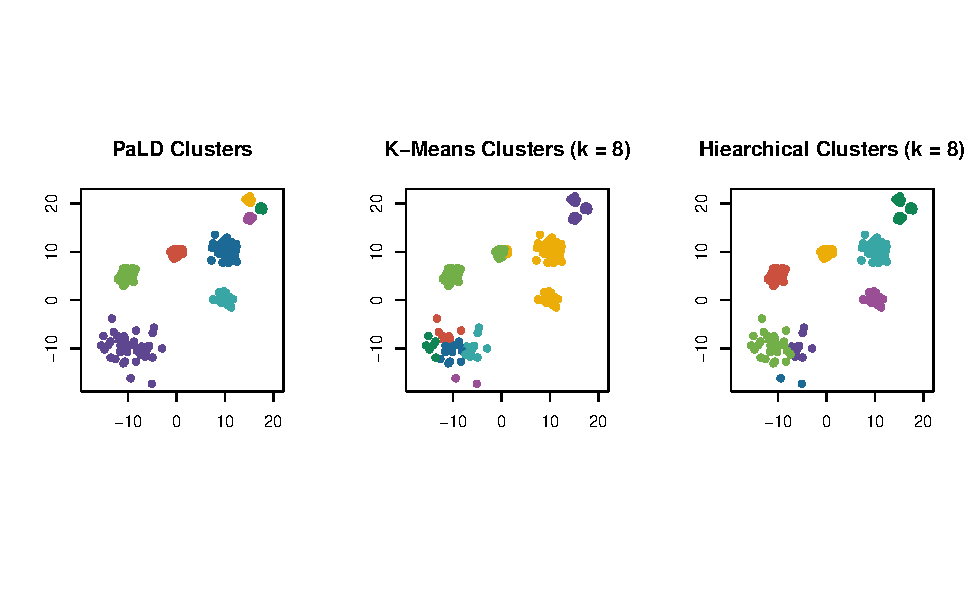
\includegraphics{dagostino-mcgowan_files/figure-latex/fig5-1} \caption[PaLD clustering of randomly generated example data (from Figure 4D from Berenhaut et al]{PaLD clustering of randomly generated example data (from Figure 4D from Berenhaut et al. (2022)) compared to k-means and hierarchical clustering with k = 8.}\label{fig:fig5}
\end{figure}
\end{Schunk}

Cohesion is particularly useful when considering data with varying local
density, see discussion in \citet{berenhaut2022social}. Note that the
PaLD algorithm is able to detect the eight natural groups within the
data without the use of any additional inputs (e.g., number of clusters)
nor optimization criteria. Despite the user input of the ``correct''
number of clusters (i.e., \(k = 8\)) both \emph{k}-means and
hierarchical clustering did not give the desired result. For further
examples, discussion, and theoretical results, see
\citet{berenhaut2022social}.

\hypertarget{summary}{%
\subsection{Summary}\label{summary}}

This paper introduces the \CRANpkg{pald} package, demonstrating its
utility for providing parameter-free clustering which can easily be
implemented for a variety of data sets. We provide example code as well
as compare the method to commonly used clustering techniques,
\emph{k}-means and hierarchical clustering.

\bibliography{RJreferences}


\address{%
Lucy D'Agostino McGowan\\
Wake Forest University\\%
Winston-Salem, NC\\ 27106\\
%
%
%
\href{mailto:mcgowald@wfu.edu}{\nolinkurl{mcgowald@wfu.edu}}%
}

\address{%
Katherine Moore\\
Wake Forest Unversity\\%
Winston-Salem, NC\\ 27106\\
%
%
%
\href{mailto:mooreke@wfu.edu}{\nolinkurl{mooreke@wfu.edu}}%
}

\address{%
Kenneth Berenhaut\\
Wake Forest University\\%
Winston-Salem, NC\\ 27106\\
%
%
%
\href{mailto:berenhks@wfu.edu}{\nolinkurl{berenhks@wfu.edu}}%
}
